\chapter{RC 1}
%\lecture{3}{22 Sep. 18:30}{Temp}
\recitation{1}{29 Sep. 18:30}{}

\section{Review}
\subsection{Axioms of Probability}
A \textbf{probability space} is a triple \(\Omega,\mathcal{\MakeUppercase{f}},P\) that contains  
\begin{itemize}
	\item The \textbf{sample space} \(\Omega \) contains all possible outcome.  
	\item The \(\sigma\)-algebra \(\mathcal{\MakeUppercase{f}} \) is the \textbf{event space}. It is a subset of the power set of \(\Omega \) we are interested in. 
	\item The \textbf{probability measure} \(P\)
	
\end{itemize}
\subsection{Probability (measure)}
\begin{itemize}
    \item The \textbf{probability measure} \(P\) is a function \(P:\mathcal{\MakeUppercase{f}} \to [0,1] \) that satisfies the three axioms. 
	\begin{enumerate}
		\item \(P(\Omega ) = 1\) 
		\item Non-negative
		\item Countable additivity for disjoint sets in \(\mathcal{\MakeUppercase{f}} \).  
	\end{enumerate}
\end{itemize}
\subsection{\(\sigma\)-algebra }
\(\mathcal{\MakeUppercase{f}} \) is call a \(\sigma\)-algebra on a set \(\Omega \) If    
\begin{enumerate}
    \item \(\emptyset \in \mathcal{\MakeUppercase{f}} \)
    \item If \(A \in \mathcal{\MakeUppercase{f}} \implies A^c \in \mathcal{\MakeUppercase{f}} \) 
    \item If \(A_1, A_2, \dots \in \mathcal{\MakeUppercase{f}} \), then \(\cup_{i = 1} A_i \in \mathcal{\MakeUppercase{f}}\) 
\end{enumerate}
\begin{eg}
    Let \(\Omega  = \{1,2,3,4,5,6\}\), find a minimal* \(\sigma\)-algebra that contains the sets \(\{1,2,3\},\{1\}\)  
\end{eg}
    Answer: \footnote[1]{\(\mathcal{\MakeUppercase{F}} =  \{\emptyset,\Omega ,\{1\},\{1,2,3\},\{4,5,6\},\{2,3,4,5,6\},\{2,3\},\{1,4,5,6\}\}\) }

\subsection{Conditional Probability}
For the general definition, take events \(A, B,\quad\) and assume that \(P(B) > 0\). The \textit{conditional probability} of the event \(A\) given \(B\) equals 
\[
    P(A|B) = \frac{P(A\cap B)}{P(B)}
\]
TBD (an example)    
\subsection{Independence}

\begin{eg}[Pairwise Independence but not independent variables]
    
\end{eg}
\section{Problem}
\begin{figure}[h]
    \centering
    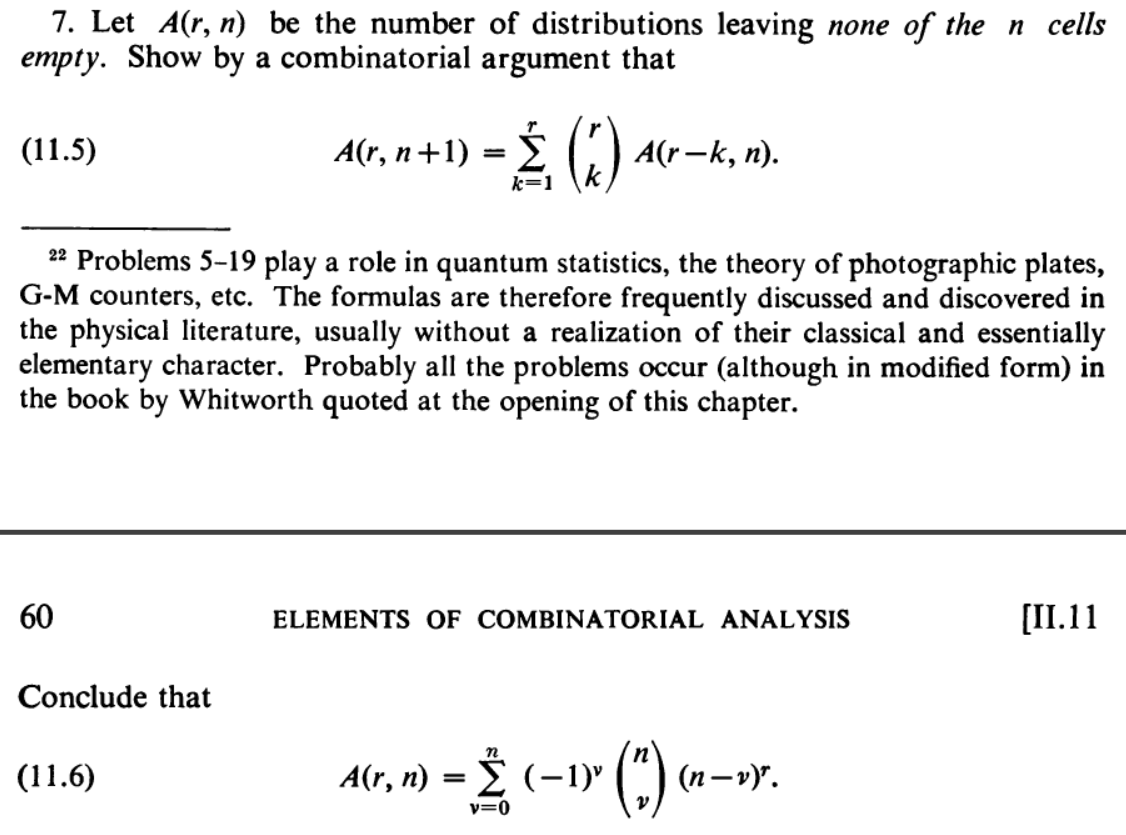
\includegraphics[width=\textwidth]{Figures/rc1_f1.png}
    \label{fig:rc1_1}
\end{figure}
\begin{figure}[h]
    \centering
    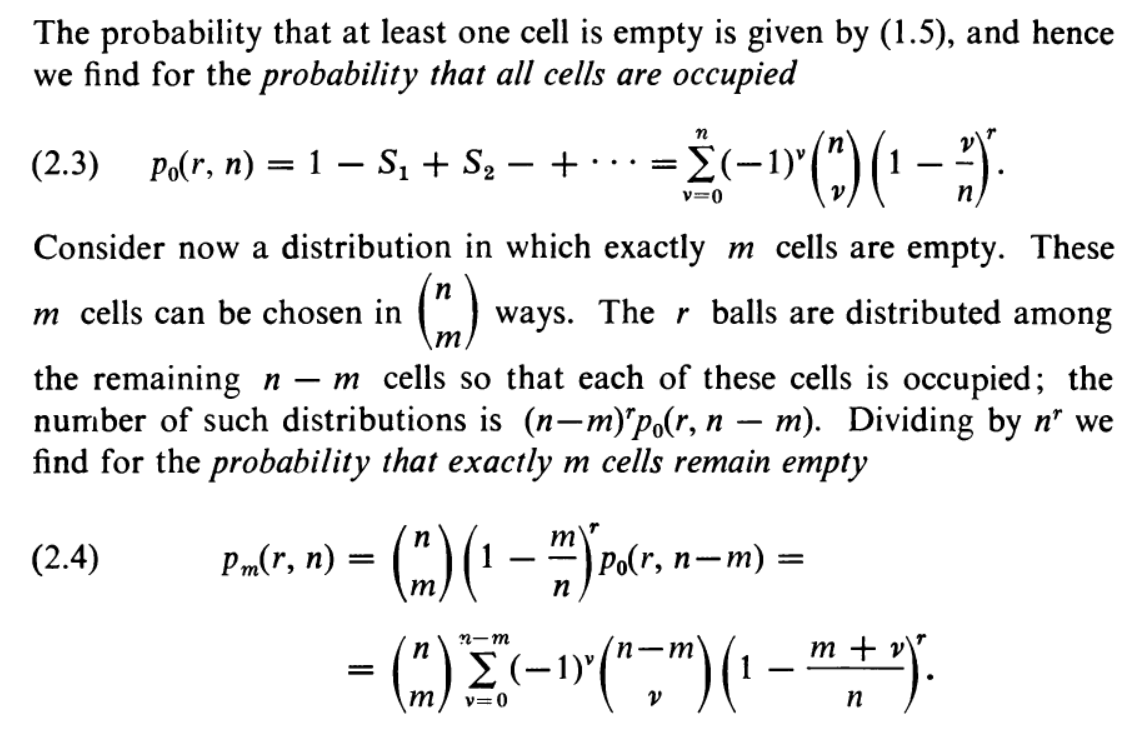
\includegraphics[width=\textwidth]{Figures/rc1_f2.png}
    \caption{A problem in Feller}
    \label{fig:rc1_2}
\end{figure}
